% funzione_gamma.tex
%! TeX root = ../lezione_turbo.tex
\Chapter{Funzione Gamma di Eulero}{"La più bella funzione dell'analisi matematica" \footnote{Come reference, si consiglia \textit{Emil Artin, The Gamma Function}}}

\begin{Def} 
Per funzione Gamma di Eulero si intende l'applicazione $ \Gamma:(0,+ \infty) \to \mathbb{R}$ data da
	\begin{equation*}
		\Gamma(x)= 
		\int_{0}^{+ \infty}e^{-t} \,t^{ \,x-1} \, \mathrm{d}t.
	\end{equation*}
\end{Def}
Osserviamo che la definizione è ben posta: l'integrabilità impropria dell'integranda è immediata sia in un intorno di $+ \infty$ che in uno di $0$ per ogni $t$ reale.

Iniziamo dalla derivabilità. 
Assumendo che certe ipotesi di regolarità siano soddisfatte, la catena di uguaglianze
\begin{equation*}
\begin{split}
	\Gamma'(x) 
	&= 
	\frac{ \partial}{ \partial x} \int_{0}^{+ \infty} e^{-t} \,t^{ \,x-1} \, \mathrm{d}t = 
	\int_{0}^{+ \infty} \frac{ \partial}{ \partial x} \left(e^{-t} \,t^{ \,x-1} \right) \, \mathrm{d}t = 
	\\ &= 
	\int_{0}^{+ \infty} e^{-t} \,t^{ \,x-1} \log t \, \mathrm{d}t
\end{split}
\end{equation*}
determina la prima derivata. 
Induttivamente, si ottiene che
\begin{equation*}
	\Gamma^{(n)}(x) = 
	\int_{0}^{+ \infty} e^{-t} \,t^{ \,x-1} \log^n t \, \mathrm{d}t,
\end{equation*}
dove l'integrabilità per ogni $n$ garantisce che $ \Gamma$ sia di classe $C^{ \infty}$. 
In particolare, la funzione è derivabile e per $x=1$ si ottiene un risultato degno di nota:
\begin{equation*}
	\Gamma'(1)= 
	\int_{0}^{+ \infty} \log t \, e^{-t} \, \mathrm{d}t = 
	- \gamma.
\end{equation*}
Riportiamo, senza dimostrazione, che la funzione è addirittura analitica. 

%%%%%%

Passiamo alla convessità. 
Nel seguito, utilizzeremo la disuguglianza di Young:
\begin{equation}
	\label{young_ineq}
	ab \leq \lambda a^ \frac{1}{ \lambda} + (1- \lambda) b^ \frac{1}{1- \lambda},	
\end{equation}
dove $a,b \in \mathbb{R}$ e $ \lambda \in \left(0,+ \infty \right)$. 

La si può dimostrare utilizzare la convessità dell'esponenziale e le sue proprietà:
\begin{equation*}
\begin{split}
	ab 
	& = 
	\exp \left( \log a + \log b \right) = 
	\exp \left({ \lambda \log a^ \frac{1}{ \lambda} + \left(1- \lambda \right) \log b^ \frac{1}{1- \lambda}} \right) \leq 
	\\ & \leq \lambda \exp \left( \log a^ \frac{1}{ \lambda} \right) + \left(1- \lambda \right) \exp \left( \log b^ \frac{1}{1- \lambda} \right) = 
	\lambda a^ \frac{1}{ \lambda} + \left(1- \lambda \right) b^ \frac{1}{1- \lambda}.
\end{split}
\end{equation*}
La convessità di $ \Gamma$, equivalente alla disuguglianza
\begin{equation*}
	\Gamma( \lambda a + (1- \lambda) b) \leq \lambda \Gamma(a) + (1- \lambda) \Gamma(b)
\end{equation*}
per ogni $a,b \in \left(0,+ \infty \right)$ e $ \lambda \in \left(0,+ \infty \right)$, segue dalla catena di relazioni
\begin{equation*}
\begin{split}
	\Gamma( \lambda a + (1- \lambda) b) 
	&= 
	\int_{0}^{+ \infty}e^{-t} \,t^{ \lambda a + (1- \lambda) b -1} \, \mathrm{d}t = 
	\\ &= 
	\int_{0}^{+ \infty}e^{-t} \,t^{ \lambda (a-1) + (1- \lambda) (b-1)} \, \mathrm{d}t \leq
	\\ &\leq 
	\int_{0}^{+ \infty}e^{-t} \left( \lambda t^{a-1} + (1- \lambda) t^{b-1} \right) \, \mathrm{d}t =
	\\ &=
	\lambda \Gamma(a) + (1- \lambda) \Gamma(b).
\end{split}
\end{equation*}
Ci sono poi alcuni punti in cui è facile computare il valore della funzione.
Nel punto $x=1$ abbiamo 
\begin{equation*}
	\Gamma(1)= 
	\int_{0}^{+ \infty}e^{-t} \, \mathrm{d}t= \left[ e^{-t} \right]_0^{+ \infty}=
	1.
\end{equation*}

Per $x=2$, invece, è sufficiente integrare per parti. Infatti, 
\begin{equation*}
	\Gamma(2) =
	\int_{0}^{+ \infty} te^{-t} \, \mathrm{d}t =
	\left[ - \frac{t}{e^t} \right]_0^{+ \infty} + \int_{0}^{+ \infty} e^{-t} \, \mathrm{d}t =
	\Gamma(1) =
	1.
\end{equation*}

Terminiamo la descrizione qualitativa della funzione con i limiti
\begin{equation*}
	\lim \limits_{x \to0^+} \Gamma(x) =
	+ \infty \qquad \lim \limits_{x \to+ \infty} \Gamma(x) =
	+ \infty,
\end{equation*}
e ricaviamo che il grafico
\begin{figure}
	\centering
	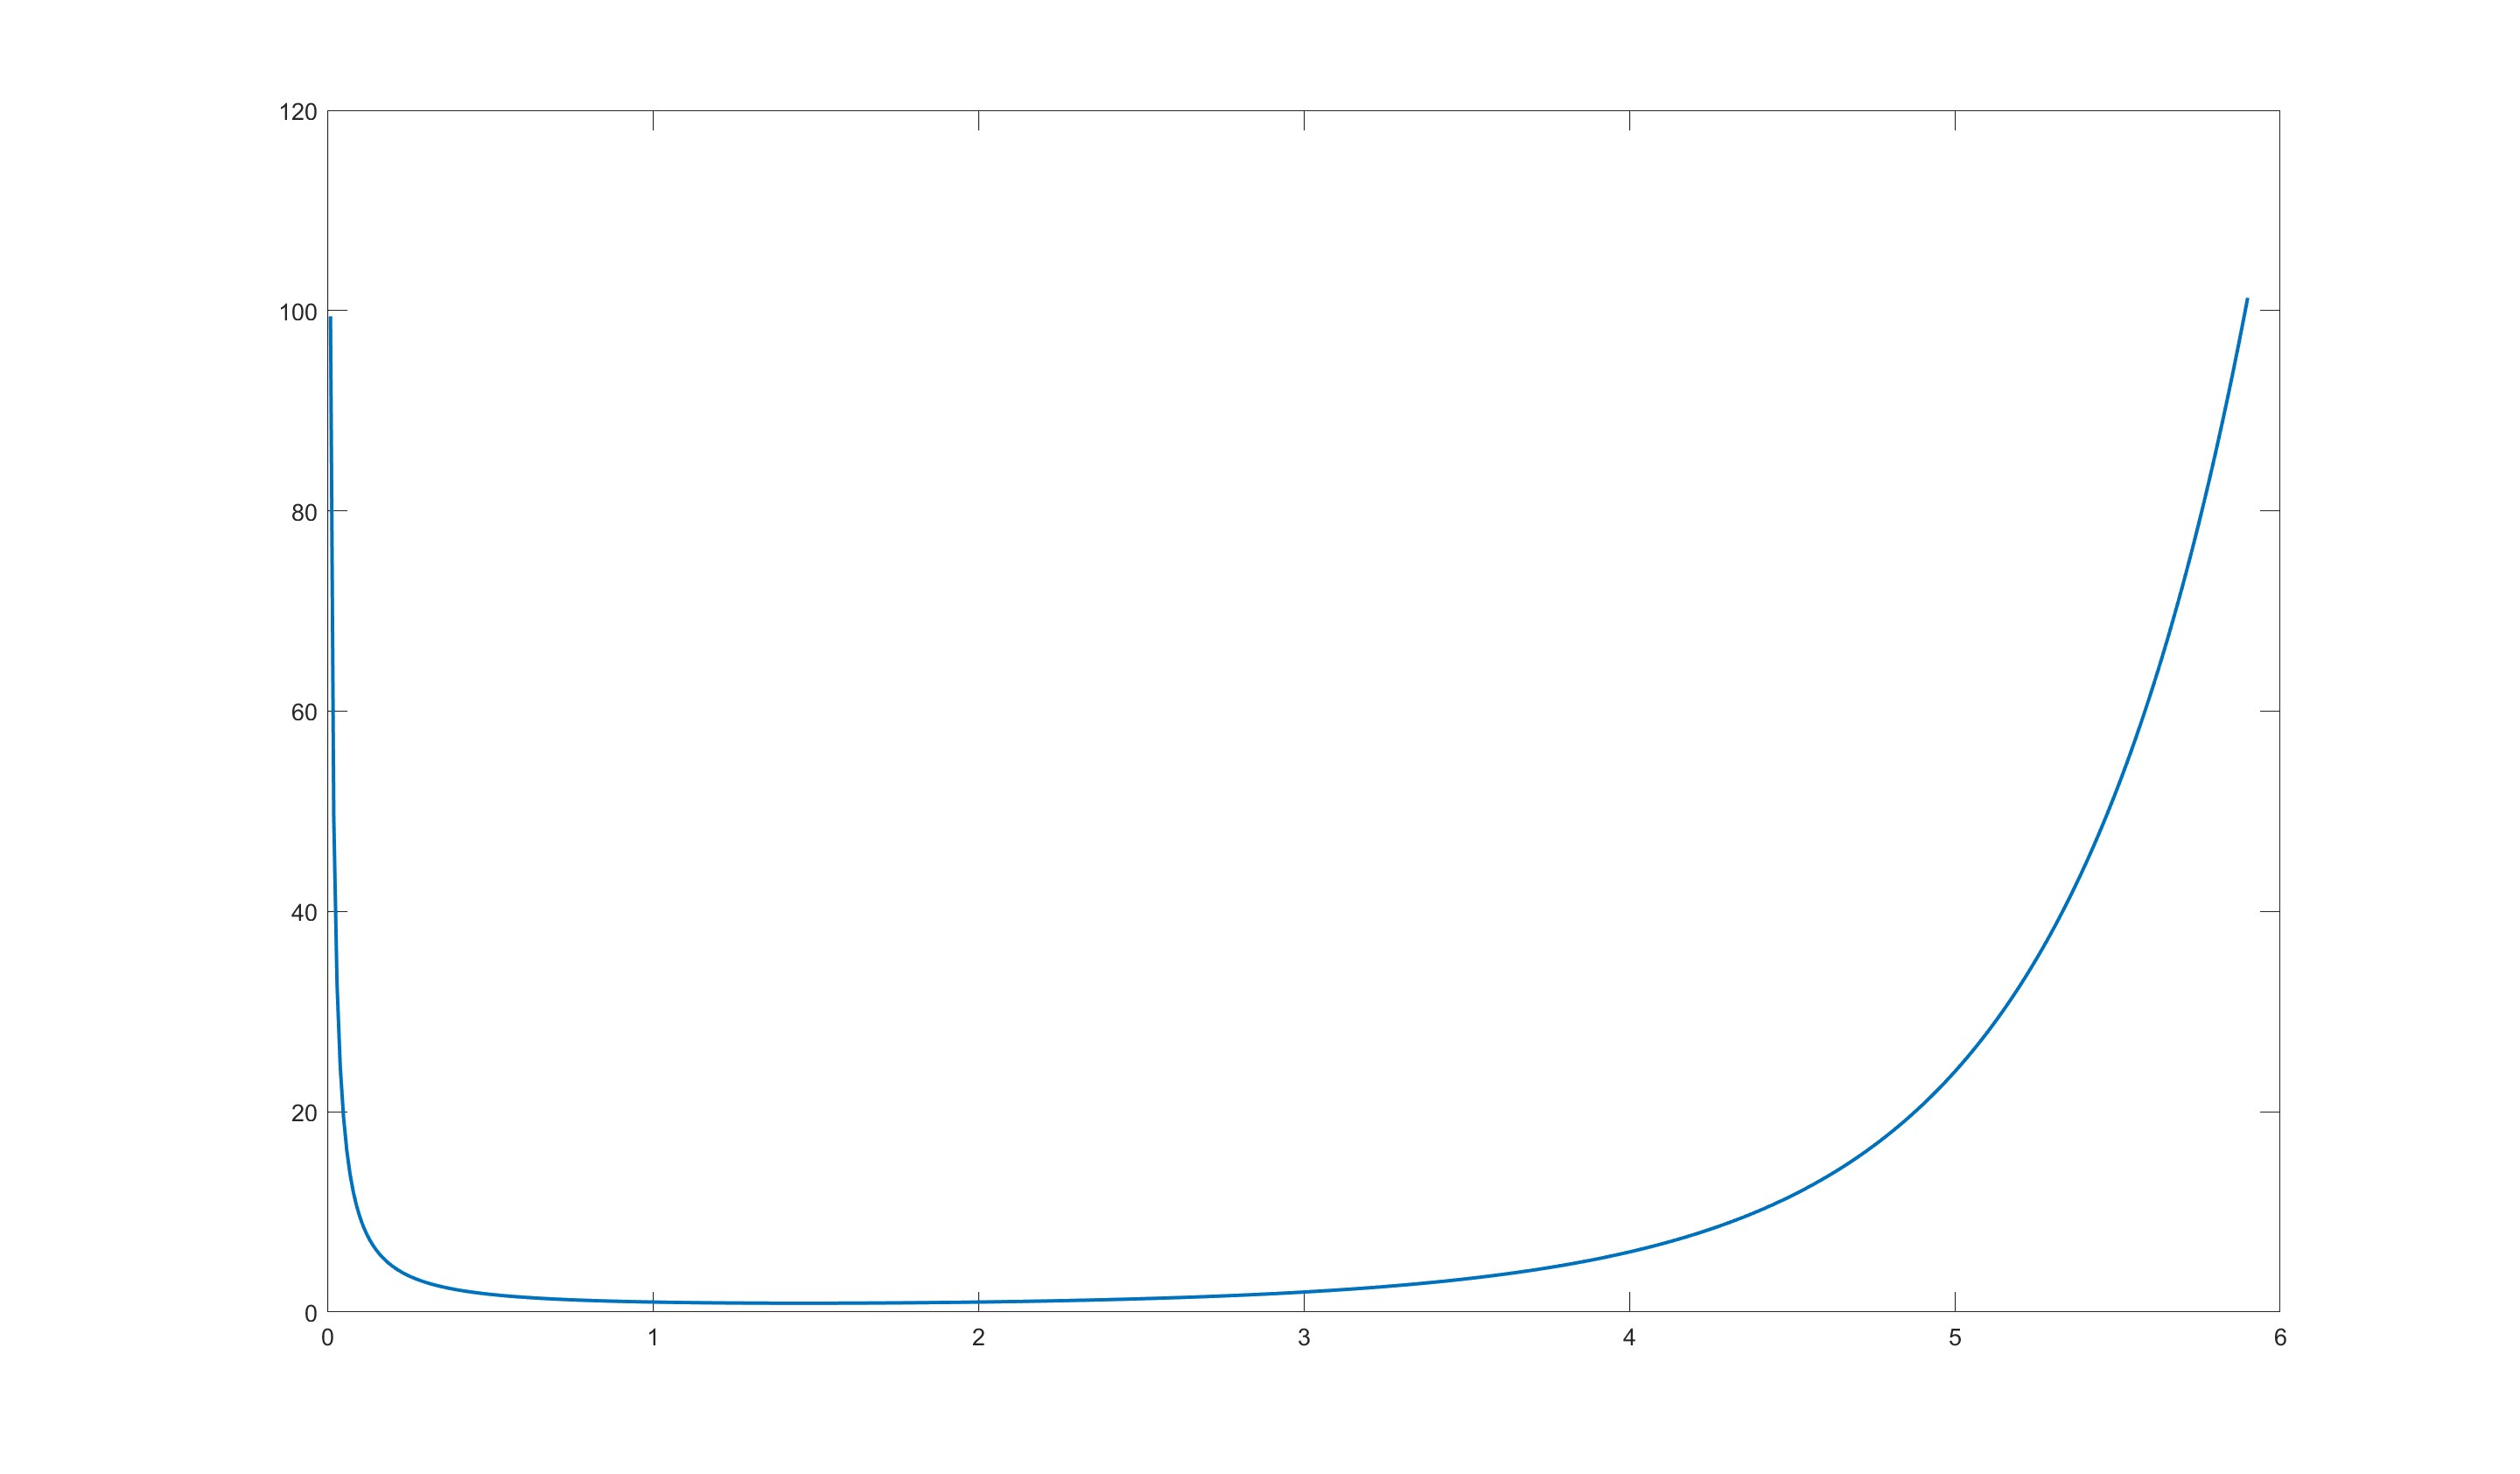
\includegraphics[width=.9\textwidth]{assets/gamma_graph.jpg}
	\caption{Grafico della funzione Gamma realizzato con MATLAB®.}
\end{figure}

La funzione è continua in $[1,2]$, e quindi per Weierstrass deve ammettere un minimo in questo intervallo. 
Poichè se esiste, a causa della monotonia della derivata il minimo deve essere anche unico, e poichè $ \Gamma(1)= \Gamma(2)$, dal Teorema di Lagrange e dal Teorema di Fermat segue che il punto di minimo della funzione è compreso tra $1$ e $2$. 
Numericamente, si trova che esso è nel punto $x_{ \min}=1,46 \dots$, con minimo $f(x_{ \min})=0,88 \dots$.

Veniamo alla relazione fondamentale del capitolo. 
\begin{Res}[Equazione funzionale della Funzione Gamma]
La funzione $ \Gamma: \mathbb{R} \to \mathbb{R}$ soddisfa l'equazione funzionale
	\begin{equation*}
		\Gamma(x+1)=
		x \Gamma(x).
	\end{equation*}
\end{Res}
\begin{proof}
È sufficiente integrare per parti (in modo tale da diminuire grado della potenza nell'integranda) per ricondursi alla tesi:
	\begin{equation*}
		\Gamma(x+1)= \int^{+ \infty}_0 e^{-t}t^x \: \, \mathrm{d}t =
		\int^{+ \infty}_0 x \, e^{-t}t^{x-1} \: \, \mathrm{d}t - \left[e^{-t}t^x \right]^{+ \infty}_0 =
		x \Gamma(x).
	\end{equation*}
\end{proof}
Voglio spendere due parole sull'idea, ricorrente, usata in questa dimostrazione. 
Propriamente, si usa l'identità di integrali propri
\begin{equation*}
	\int^L_0 e^{-t} t^x \: \, \mathrm{d}t = 
	\int^L_0 x \, e^{-t} t^{x-1} \: \, \mathrm{d}t - \left[e^{-t} t^x \right]^L_0,
\end{equation*}
valutata al limite. 
Questa, presenta due termini: uno che si stabilizza al crescere di $L$, e l'altro si annulla. 
In altri termini, man mano che l'intervallo su cui consideriamo l'integrale si "globalizza", il termine di bordo decade \footnote{Gli audaci che dovessero usare il Griffith per Fisica 2, riconosceranno l'uso di questa tecnica.}.

Tornando a noi, un'applicazione immediata dell'Equazione Funzionale è che possiamo valutare la velocità di divergenza.
In $x=0$,
\begin{equation*}
	\Gamma(x)= \frac{ \Gamma(x+1)}{x} \sim \frac{1}{x}
\end{equation*}
Pertanto, $ \Gamma$ diverge come la funzione $ \frac{1}{x}$ in quell'intorno. 

Valutare l'asintotico all'infinito è più difficile. 
Per farlo, partiamo da una valutazione della funzione su una classe di punti.

\begin{Res}[Valutazione nei naturali della Funzione Gamma] 
La funzione reale $ \Gamma(x)$ interpola la funzione fattoriale che ha per dominio $ \mathbb{N}$. 
In altri termini,
	\begin{equation*}
		\Gamma(n+1)=n! \quad \forall n \in \mathbb{N}.
	\end{equation*}
\end{Res}
\begin{proof}
Immediato per induzione, con caso base $ \Gamma(1)=1$.
\end{proof}
Anche se provato solo successivamente, possiamo fare ipotesi sulla velocità di crescita di $ \Gamma$: non soprenderà nessuno che valga proprio l'asintotico $ \Gamma(x) \sim x^x e^{-x} \sqrt{2 \pi x}$.


Anche altre valutazioni analitiche sono possibili grazie a questo strumento. 
Osservando che in $x= \frac{1}{2}$, attraverso la sostituzione $y^2=t$, ci si riconduce immediatamente all'integrale di Gauss, otteniamo 
\begin{equation*}
	\Gamma \left( \frac{1}{2} \right)= \int_{0}^{+ \infty}e^{-t}t^{- \frac{1}{2}} \, \mathrm{d}t=2 \int_{0}^{+ \infty}e^{-y^2} \, \mathrm{d}y= \sqrt{ \pi}.
\end{equation*} 
Utilizzando la relazione funzionale possiamo valutare $ \Gamma$ per altri valori.
\begin{Res}[Valutazione nei numeri $n+ \frac{1}{2}$ della Funzione Gamma] Per $n \in \mathbb{N}$,
	\begin{equation*}
		\Gamma \left(n+ \frac{1}{2} \right) = 
		\sqrt{ \pi} \frac{(2n)!}{4^n n!}.
	\end{equation*}
\end{Res}

Solo il seguente risultato, il teorema di Bohr-Mollerup, sottolinea però la vera forza di questa relazione. 
L'unico prerequisito per comprenderne l'enunciato è la nozione di $ \log$-convessità: si tratta di una condizione di regolarità più forte della convessità, per cui anche il logaritmo della funzione è convesso. 
Un esercizio è dimostrare che questa condizione implica la convessità. 
Senza dimostrazione \footnote{Rudin, Principles of Mathematical Analysis, Teorema 8.18.}, affermiamo che la funzione Gamma è $ \log$-convessa.

\begin{The}[Bohr-Mollerup]
Sia $f:(0,+ \infty) \to(0,+ \infty)$ tale che
\begin{enumerate}
	\item f(1)=1,
	\item soddisfi f(x+1)=xf(x),
	\item f è $ \log$-convessa.
\end{enumerate}
Allora, la funzione è unicamente determinata da
\begin{equation*}
f(x) = 
\lim_{n \to \infty} \frac{n^x n!}{x(x+1) \dots(x+n)}.	
\end{equation*}
\end{The}
Quindi, la funzione $ \Gamma$, $ \log$-convessa che soddisfa (2), è anche l'unica con queste proprietà. 
Il teorema fornisce inoltre una caratterizzazione \footnote{Termine da matematico per "maniera di indicare un oggetto senza ambiguità, e cioè unicamente, descrivendolo attraverso delle proprietà diverse da quelle con cui è stato definito". 
Comunemente usato in Probabilità, Teoria della Misura e Geometria.} alternativa, come limite
\begin{equation*}
	\Gamma(x) = 
	\lim_{n \to \infty} \frac{n^x n!}{x(x+1) \dots(x+n)}.	
\end{equation*}

\pagebreak